%{{{-----------------------------------Basics----------------------------------%

%{{{document class definition
\documentclass[
    11pt,
    a4paper,
    oneside,
    headinlcude, footinclude,
    twoside,
]{report}
%}}}

%{{{essential packages
\renewcommand*\rmdefault{ppl}
\usepackage[top=2.5cm,bottom=2.5cm,left=3cm,right=3cm]{geometry}
\usepackage[english]{babel}
\usepackage[T1]{fontenc}
\usepackage[utf8]{inputenc}
\usepackage{xcolor}
\usepackage{amssymb}
%}}}

%{{{additional packages
\usepackage{amssymb}
\usepackage{amsmath}
\usepackage{mathtools}
\usepackage[framemethod=Tikz]{mdframed}
\usepackage{tikz}
\usepackage{enumerate}
\usepackage{graphicx}
\usepackage{pgf,tikz,pgfplots} % for the transfer from geogebra to tikz
\usepackage{mathrsfs}% for the transfer from geogebra to tikz
\usepackage{stackrel}
\usepackage{fancyhdr}
\usepackage{tabularx}
\usepackage{makecell} % to make thick hlines in the front page
\usepackage{centernot}
\usepackage[makeroom]{cancel}
%}}}

%}}}

%{{{-----------------------------------Macros----------------------------------%

\newcommand{\myImplies}[0]{\rightarrow}

\newcommand{\powerset}[1]{\mathcal{P}(#1)}

\newcommand{\tvect}[3]{%
   \ensuremath{\Bigl(\begin{smallmatrix}#1\#2\#3\end{smallmatrix}\Bigr)}}

\newcommand{\myVector}[3]{\begin{pmatrix}#1\#2\#3\end{pmatrix}}

\newcommand{\tq}[0]{\textrm{ t.q. }}

\newcommand{\markDate}[1]{\begin{flushright}#1\end{flushright}}

\newcommand{\cqfd}[0]{\begin{flushright}$\Box$\end{flushright}}

\renewcommand{\vec}[1]{\overrightarrow{#1}}

\def\getangle(#1)(#2)#3{
    \begingroup
        \pgftransformreset
        \pgfmathanglebetweenpoints{\pgfpointanchor{#1}{center}}{\pgfpointanchor{#2}{center}}
        \expandafter\xdef\csname angle#3\endcsname{\pgfmathresult}
    \endgroup
}

%colored frame box
\newcommand{\cfbox}[2]{
    \colorlet{currentcolor}{.}
    {\color{#1}
    \fbox{\color{currentcolor}#2}}
}

\newcommand\Warning{
    \makebox[1.4em][c]{
    \makebox[-5.5pt][c]{\raisebox{.2em}{!}}
    \makebox[0pt][c]{\color{red}\huge$\bigtriangleup$}}
}

%}}}

%{{{----------------------------------Settings---------------------------------%

\title{Maths 1B - Analyse}

\author{Arnò Fauconnet}

\setlength{\parindent}{0pt} %disable initial indent on first paragraph of sections in the whole doc

% the style of the boxes
\newmdenv[
        roundcorner=10pt,
        middlelinecolor=red,
        backgroundcolor=gray!15,
        linewidth=2pt,
        frametitlerule=true]{highlightBox}

% increases the space between paragraphs
\setlength{\parskip}{.3em}

%\setlength{\headheight}{15pt}

% geogebra library usage
\usetikzlibrary{arrows}
\pgfplotsset{compat=1.15}

% Geogebras wierd colors xD
\definecolor{qqqqff}{rgb}{0.,0.,1.}
\definecolor{ffqqtt}{rgb}{1.,0.,0.2}
\definecolor{ududff}{rgb}{0.30196078431372547,0.30196078431372547,1.} 
\definecolor{ffqqqq}{rgb}{1.,0.,0.} 
\definecolor{xdxdff}{rgb}{0.49019607843137253,0.49019607843137253,1.}
\definecolor{zzttqq}{rgb}{0.6,0.2,0.}
\definecolor{uuuuuu}{rgb}{0.26666666666666666,0.26666666666666666,0.26666666666666666}
\definecolor{qqzzqq}{rgb}{0.,0.6,0.}
\definecolor{ccqqqq}{rgb}{0.8,0.,0.}
\definecolor{qqwuqq}{rgb}{0.,0.39215686274509803,0.}
\definecolor{wwqqcc}{rgb}{0.4,0.,0.8}

\graphicspath{ {Maths_1B/figures/} }

%\tikzstyle{every node}[font=\large]


% header and footer settings
\pagestyle{fancy}
\fancyhf{}
\fancyhead[LE,LO]{Arnaud Fauconnet}
\fancyhead[CE,CO]{\textsc{Maths 1B}}
\fancyhead[RE,RO]{MAN - Printemps 2019}
\fancyfoot[CE,CO]{\leftmark}
\fancyfoot[LE,RO]{\thepage}

\renewcommand{\headrulewidth}{2pt}
\renewcommand{\footrulewidth}{1pt}

%}}}

%%%%%%%%%%%%%%%%%%%%%%%%%%%%%%%%%%%%%%%%%%%%%%%%%%%%%%%%%%%%%%%%%%%%%%%%%%%%%%
%----------------------------------------------------------------------------%
%-------------------------------Text starts here-----------------------------%
%----------------------------------------------------------------------------%
%%%%%%%%%%%%%%%%%%%%%%%%%%%%%%%%%%%%%%%%%%%%%%%%%%%%%%%%%%%%%%%%%%%%%%%%%%%%%%


\begin{document}

\begin{titlepage}
   \begin{center}
       \vspace*{\fill}

       {\Huge EPFL}\\ 
%----------------------------------------------------------------------------%
       \vfill
       {\huge MAN}\\ [1em]
       {\Large Mise à niveau}\\
%----------------------------------------------------------------------------%
        \vfill
        \begin{tabularx}{\textwidth}{X}
            \Xhline{3\arrayrulewidth}\\
        \end{tabularx}\\ [2em]
        {\Huge Maths 1B} \\ [1em]
        \textsc{\huge Prepa-033(b)} \\ [2em]
        \begin{tabularx}{\textwidth}{X}
            \Xhline{3\arrayrulewidth}\\
        \end{tabularx}\\ [2em]
%----------------------------------------------------------------------------%
        \vspace{.7cm}
        {\large
        \begin{tabularx}{.9\textwidth}{Xr}
            \textit{Student:} & \textit{Professor:}\\
            Arnaud \textsc{Fauconnet} & Olivier \textsc{Woringer}
        \end{tabularx}}
%----------------------------------------------------------------------------%
        \vfill
        {\Large Printemps - 2019}

%----------------------------------------------------------------------------%
        \vfill
        \includegraphics[width=7cm]{epfl-logo}

       \vfill
   \end{center} 
\end{titlepage} 
\setcounter{chapter}{2}
\chapter{Calcul différentiel}
\label{cha:calcul_differentiel}

\section{Dérivée d'une fonction}
\label{sec:derivee_d_une_fonction}


\subsection{Définitions}
\label{sub:definitions}

Soit $f$ définie sur un voisinage de $x_{0}$, posons $y = f(x)$. Une
information \textbf{locale} sur le comportement de $f$ sur un voisinage de $x_{0}$
est donné par le quotien $$\frac{\Delta y}{\Delta x} = \frac{f(x_{0} + \Delta x )
- f(x_{0})}{(x_{0} + \Delta x ) - x_{0}}$$
appelé le rapport de Newton de $f$ en $x_{0}$.

\begin{itemize}
    \item $\Delta x $ est l'accroissement de la variable indépendante $x$.
    \item $\Delta y$ est l'accroissement correspondant liée à $\Delta x $.


\end{itemize}

\begin{center}
    \begin{minipage}{.5\linewidth}
        \resizebox{\textwidth}{!}{
            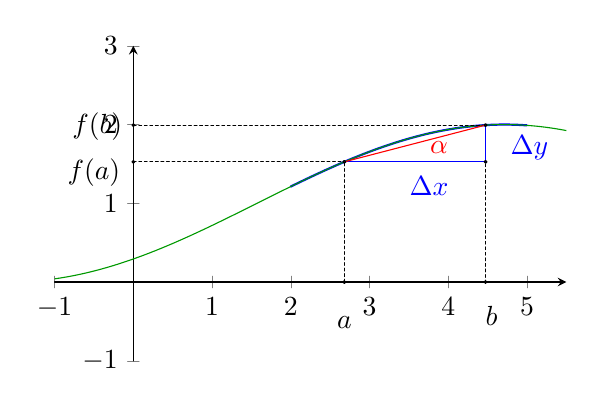
\begin{tikzpicture}[line cap=round,line join=round,>=triangle 45,x=1.0cm,y=1.0cm]
            \begin{axis}[
            x=1.0cm,y=1.0cm,
            axis lines=middle,
            xmin=-1.0,
            xmax=5.5,
            ymin=-1.0,
            ymax=3.0,
            xtick={},
            ytick={},]
            \clip(-1.,-1.) rectangle (5.5,3.);
            \draw[line width=.8pt,color=qqqqff,samples=100,domain=2:5] plot(\x,{cos(0.5*(\x + 2.5*3.14159265358979323)*180/pi)+1});

            \draw[line width=0.4pt,color=qqzzqq,smooth,samples=100,domain=-1.0:5.5] plot(\x,{cos((1.0/2.0*((\x)+2.5*3.141592653589793))*180/pi)+1.0});
            \draw [line width=0.4pt,dash pattern=on 1pt off 1pt] (0.,1.5264006802392824)-- (2.6795196769160747,1.5264006802392824);
            \draw [line width=0.4pt,dash pattern=on 1pt off 1pt] (0.,1.9928404338545378)-- (4.4729208075480695,1.9928404338545378);
            \draw [line width=0.4pt,dash pattern=on 1pt off 1pt] (4.4729208075480695,1.9928404338545378)-- (4.4729208075480695,0.);
            \draw [line width=0.4pt,dash pattern=on 1pt off 1pt] (2.6795196769160747,0.)-- (2.6795196769160747,1.5264006802392824);
            \draw [line width=0.4pt,color=qqqqff] (2.6795196769160747,1.5264006802392824)-- (4.4729208075480695,1.5264006802392824);
            \draw [line width=0.4pt,color=qqqqff] (4.4729208075480695,1.5264006802392824)-- (4.4729208075480695,1.9928404338545378);
            \draw [line width=0.4pt,color=ffqqqq] (2.6795196769160747,1.5264006802392824)-- (4.4729208075480695,1.9928404338545378);
            \begin{scriptsize}
            \draw [fill=black] (2.6795196769160747,0.) circle (0.5pt);
            \draw[color=black] (2.681568168520954,-0.5175265875183013) node {$a$};
            \draw [fill=black] (4.4729208075480695,0.) circle (0.5pt);
            \draw[color=black] (4.548321034281871,-0.4326741845291687) node {$b$};
            \draw [fill=uuuuuu] (2.6795196769160747,1.5264006802392824) circle (0.5pt);
            \draw [fill=uuuuuu] (4.4729208075480695,1.9928404338545378) circle (0.5pt);
            \draw [fill=black] (0.,1.5264006802392824) circle (0.5pt);
            \draw[color=black] (-0.5003969435715185,1.391652479737182) node {$f(a)$};
            \draw [fill=black] (0.,1.9928404338545378) circle (0.5pt);
            \draw[color=black] (-0.45797074207695215,1.9714772334962547) node {$f(b)$};
            \draw [fill=qqqqff] (4.4729208075480695,1.5264006802392824) circle (0.5pt);
            \draw[color=qqqqff] (3.756365273049967,1.2219476737589168) node {$\Delta x$};
            \draw[color=qqqqff] (5.0291513178869565,1.7027779573640016) node {$\Delta y$};
            \draw[color=ffqqqq] (3.883643877533666,1.7027779573640016) node {$\alpha$};
            \end{scriptsize}
            \end{axis}
            \end{tikzpicture}
        }
    \end{minipage}
    \begin{minipage}{.49\linewidth}
        \setlength{\parskip}{.3em}

        $$\frac{\Delta y}{\Delta x } = \tan(x) \text{ est la pente }$$
        
        sécente passant par $(x_{0}, f(x_{0}))$ et $(x_{0} + \Delta x; f(x_{0}
        + \Delta x ))$
    \end{minipage}
\end{center}

En gardant $x_{0}$ fixe, on fait tendre $\Delta x \to 0$

Alors $$x_{0} + \Delta x \to x_{0}$$
et $$f(x_{0} + \Delta x) \to f(x_{0})$$
si $f$ est continue en $x_{0}$, alors $$\frac{\Delta y}{\Delta x}$$
est une FI de type $"\frac{0}{0}"$

Trois cas peuvent se présenter
\begin{enumerate}
    \item $\lim\limits_{\Delta x \to 0}\frac{\Delta y}{\Delta x}$ n'existe pas 
        \paragraph{Exemple:}
        
        $$ f(x) = \left\{
            \begin{array}{ll}
            x \cdot \sin(x) & \text{ si } x \neq 0\\
            0 & \text{ si } x = 0\\
            \end{array}
        \right., \quad x_{0} = 0$$
    \item $\lim\limits_{\Delta x \to 0}\frac{\Delta y}{\Delta x} = + \infty$

        \paragraph{Exemple:}
        
        $$f(x) = \sqrt[3]{x^{3} + x}, \quad x_{0} = 0$$

    \item $\lim\limits_{\Delta x \to 0}\frac{\Delta y}{\Delta x} = a, \quad (a
        \in \mathbb{R})$

        $$\lim_{\Delta x \to 0}\frac{\Delta y}{\Delta x} = \lim_{\Delta x \to 0}\frac{
        (2 + \Delta x )^{2} - 2^{2}}{\Delta x} = 4$$
\end{enumerate}

\paragraph{Définition:}

Soit $f$ définie sur un voisinage de $x_{0}$. On dit que $f$ est dérivable en
$x_{0}$. Si 
$$\lim_{\Delta x \to 0}\frac{\Delta y}{\Delta x}$$
existe et on note $f'(x_{0})$ cette limite.

$$f'(x_{0}) = \lim_{\Delta x \to 0} \frac{f(x_{0} + \Delta x ) - f(x_{0})}{\Delta
x}$$
est appelé \textbf{nombre dérivé} de $f$ en $x_{0}$

\begin{center}
    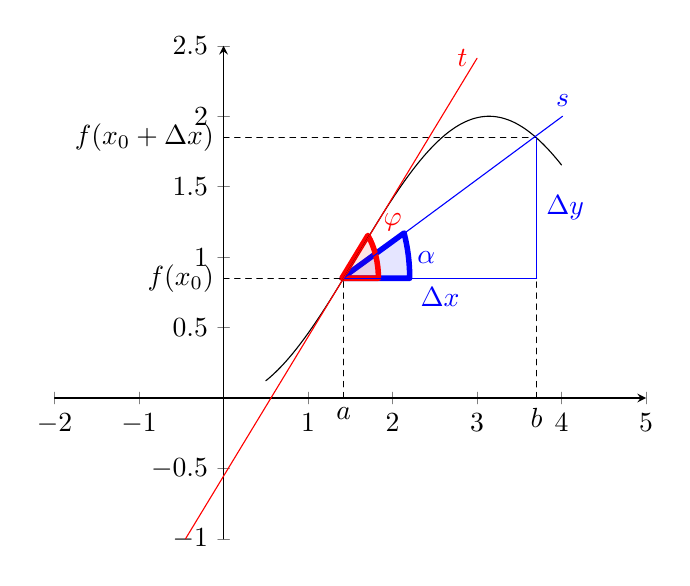
\begin{tikzpicture}[line cap=round,line join=round,>=triangle 45,x=1.0cm,y=1.0cm]
    \begin{axis}[
    width=.75\linewidth,
    axis lines=middle,
    xmin=-2.0,
    xmax=5.0,
    ymin=-1,
    ymax=2.5,
    xtick={},
    ytick={},]
    \clip(-2.,-1) rectangle (5.,2.5);
    \draw [shift={(-.6,-0.15)},line width=2.pt,color=qqqqff,fill=qqqqff,fill opacity=0.10000000149011612] (0,0) -- (0.:0.8027663949036016) arc (0.:23.572836195031222:0.8027663949036016) -- cycle;
    \draw [shift={(-.6,-0.15)},line width=2.pt,color=ffqqqq,fill=ffqqqq,fill opacity=0.10000000149011612] (0,0) -- (0.:0.43225882802501625) arc (0.:44.675027547991505:0.43225882802501625)
     -- cycle ;
    \draw[line width=0.4pt,color=black,smooth,samples=100,domain=.5:4] plot(\x,{cos(((\x)+3.141592653589793)*180/pi)+1.0});
    \draw [line width=0.4pt,dash pattern=on 2pt off 2pt] (0.,0.8502254697469851)node [anchor =east]{$f(x_{0})$}-- (1.4204560999795453,0.8502254697469851);
    \draw [line width=0.4pt,dash pattern=on 2pt off 2pt] (0.,1.8463139118229057)node [anchor =east]{$f(x_{0} + \Delta x)$}-- (3.703362039584402,1.8463139118229057);
    
    \draw [line width=0.4pt,dash pattern=on 2pt off 2pt] (3.703362039584402,1.8463139118229057)-- (3.703362039584402,0.)
    node [anchor = north] {$b$};
    \draw [line width=0.4pt,dash pattern=on 2pt off 2pt] (1.4204560999795453,0.)node [anchor = north] {$a$}-- (1.4204560999795453,0.8502254697469851);
    \draw [line width=0.4pt,color=qqqqff] (1.4204560999795453,0.8502254697469851)-- (3.703362039584402,0.8502254697469851) node [anchor=north, midway] {$\Delta x$};
    \draw [line width=0.4pt,color=qqqqff] (3.703362039584402,0.8502254697469851)-- (3.703362039584402,1.8463139118229057) node [anchor=west, midway] {$\Delta y$};
    \draw [line width=0.4pt,color=qqqqff] (1.4204560999795453,0.8502254697469851)-- (4.0116276,2)
    node [anchor = south] {$s$};
    \draw [line width=0.4pt,color=ffqqqq,domain=-1.:3.] plot(\x,{(-0.5542081380527308--0.9887201778498751*\x)/1.}) node [anchor = east] {$t$};

    \begin{scriptsize}
    \draw[color=qqqqff] (2.718281281470374,0.5742003555500957);
    \draw[color=qqqqff] (2.4,1) node {$\alpha$};
    \draw[color=ffqqqq] (-1.4437537197990677,-1.7476470635557058) node {$s$};
    \draw[color=ffqqqq] (2,1.25) node {$\varphi$};
    \end{scriptsize}
    \end{axis}
    \end{tikzpicture}
\end{center}

La sécant $s$ tends vers la "droite-limite" $t$.

$$\alpha \xrightarrow[\Delta \to 0]{} \varphi$$

Cette "droite-limite" est appelée la tangente à $$y = f(x_{0}) \text{ en } x_{0}$$
La pente $m$ de la tangente vaut $$m = \tan(\varphi) = \lim_{\Delta x \to 0} \frac{\Delta
y}{\Delta x } = f'(x_{0})$$

Donc l'équivalente de $t$ s'écrit 
\begin{highlightBox}[frametitle={Tangente de $y=f(x)$}]
    $$t: y - f(x_{0}) = f'(x_{0}) \cdot (x - x_{0})$$
\end{highlightBox}

\paragraph{Théorème:}

Soit $f$ définie sur un voisinage de $x_{0}$. Alors $$f \text{ dérivable en }
x_{0} \implies f \text{ continue en } x_{0}$$

\paragraph{Démonstration}
\label{par:demonstration}
$f$ est dérivable en $x_{0}$ donc 
\[
    \begin{split}
        &\lim_{\Delta x \to 0} \frac{f(x_{0} + \Delta x ) - f(x_{0})}{\Delta x } = f'(x_{0})\\
        \implies &\lim_{\Delta x \to 0} \underbrace{\left(\frac{f(x_{0} + \Delta x ) - f(x_{0})}{\Delta x } - f'(x_{0})\right)}_{{\color{red}
    := r(\Delta x)}} = 0\\
    \end{split}
\]

Donc $$\lim_{\Delta x \to 0} r (\Delta x) = 0$$
et $$f(x_{0} + \Delta x) = f(x_{0}) + \Delta x \cdot f'(x_{0}) + \Delta x \cdot
r(\Delta x)$$
Et lorsque $\Delta x \to 0$, on a $$\lim_{\Delta x \to 0} f(x_{0} + \Delta x)
= f(x_{0}) + \underbrace{\lim_{\Delta x \to 0} \Delta x \cdot f'(x_{0})}_{\to 0}+
\underbrace{\lim_{\Delta x \to 0} \Delta x \cdot \overbrace{r(\Delta x)}^{\to 0}}_{\to 0}$$

 $f$ est donc continue en $x_{0}$ \cqfd

\Warning La réciproque est fausse \Warning

\paragraph{Contre-exemple}
\label{par:contre_exemple}

\begin{center}
 \begin{minipage}{.4\linewidth}
     \resizebox{\textwidth}{!}{
        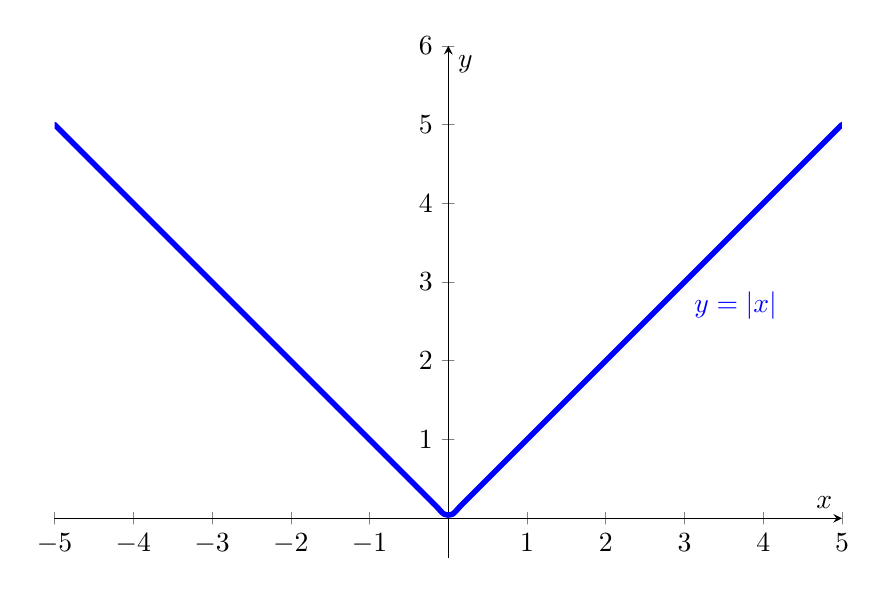
\begin{tikzpicture}[line cap=round,line join=round,>=triangle 45,x=1.0cm,y=1.0cm]
        \begin{axis}[
        x=1.0cm,y=1.0cm,
        axis lines=middle,
        xmin=-5.0,
        xmax=5.0,
        ymin=-0.5,
        ymax=6.0,
        xtick={},
        ytick={},
        xlabel={$x$},
        ylabel={$y$},]
        \clip(-5.,-0.5) rectangle (5.,6.);
        \draw[line width=2.pt,color=qqqqff,smooth,samples=100,domain=-5.0:5.0] plot(\x,{abs((\x))});
        \begin{scriptsize}
        \draw[color=qqqqff] (3,3) node [anchor = north west]{$y = |x|$};
        \end{scriptsize}
        \end{axis}
        \end{tikzpicture}
     }
 \end{minipage}
 \begin{minipage}{.59\linewidth}
     \setlength{\parskip}{.3em}
     $$f(x) = |x|, \quad x_{0} = 0, \quad \quad \lim_{x \to 0} |x| = 0, \quad |x|\Bigr|_{x = 0} = 0$$
     donc $|x|$ est continue en $x = 0$

     Mais $$\lim_{\Delta x \to 0} \frac{|0+\Delta x| - 0}{\Delta x} = \lim_{\Delta
         x\to 0} \frac{|\Delta x|}{\Delta x}$$
    n'existe pas donc $f(x) = |x|$ n'est pas dérivable en $x \to 0$.
 \end{minipage}
\end{center}


\paragraph{Définitions:}

\begin{itemize}
    \item On dit que $f$ est dérivable à gauche en $x_{0}$, si $$\lim_{x \to x_{0}^{-}} \frac{f(x) - f(x_{0})}{x - x_{0}}$$
        existe, on note ce nombre $f'(x_{0}^{-})$ et il représente la pente de
        la demi-tangente à gauche en $x_{0}$.
    \item de même  $f$ est dérivable à droite en $x_{0}$, si $$\lim_{x \to
            x_{0}^{+}} \frac{f(x) - f(x_{0})}{x - x_{0}}$$
        existe, $f'(x_{0}^{+})$ et il représente la pente de
        la demi-tangente à droite en $x_{0}$.
\end{itemize}

\paragraph{Exemple:}

\begin{center}
    \begin{minipage}{.5\linewidth}
        \resizebox{\textwidth}{!}{
            \begin{tikzpicture}[line cap=round,line join=round,>=triangle 45,x=1.0cm,y=1.0cm]
            \begin{axis}[
            x=1.0cm,y=1.0cm,
            axis lines=middle,
            xmin=-5.0,
            xmax=5.0,
            ymin=-0.5,
            ymax=4.5,
            xtick={},
            ytick={},
            xlabel={$x$},
            ylabel={$y$},
            ]
            \clip(-4.,-0.5) rectangle (4.,4.5);
            \draw[line width=0.4pt,smooth,samples=100,domain=-4.0:4.0] plot(\x,{abs((\x))});
            \draw [->,line width=0.8pt,color=qqqqff] (-3.,3.) -- (0.,0.) node [anchor = north east, midway] {$m = f(0^-) = -1$};
            \draw [->,line width=0.8pt,color=ffqqqq] (0.,0.) -- (3.,3.) node [anchor = north west, midway] {$m = f(0^+) = 1$};
            \end{axis}
            \end{tikzpicture}
        }
    \end{minipage}
    \begin{minipage}{.49\linewidth}
        \setlength{\parskip}{.3em}
        $$f(0^{-}) = - 1$$
        $$f(0^{+}) = + 1$$
    \end{minipage}
\end{center}

\paragraph{Définitions:}

Si $I \subset \mathbb{D}_{f}$
\begin{itemize}
    \item Si $f$ est dérivable en tout $x_{0} \in I$, on définit: 
        \[
            \begin{split}
                f' : I& \to \mathbb{R},\\
                x_{0}& \mapsto f'(x_{0}) = \lim_{\Delta x \to 0} \frac{f(x_{0}
            + \Delta x) - f(x_{0})}{\Delta x}
            \end{split}
        \]
        appelé la fonction dérivée de $f$ sur $I$.
    \item Si $f$ est dérivable sur $I$, et si $f'$ est continue sur $I$, alors
        on dit que $f$ est continument dérivable sur $I$ et on note $f \in
        \mathbb{C}^{1}$
\end{itemize}


\subsection{Règles de dérivation}
\label{sub:_regles_de_derivation}

(C.f. exercice facultatif série 8)

Soient $f$ et $g$ dérivable sur $I \in \mathbb{D}_{f} \cap \mathbb{D}_{g}$ 

\begin{enumerate}
    \item $(f + g)' (x) = f'(x) + g'(x)$
    \item $(\lambda \cdot f)' (x) = \lambda \cdot f'(x)$
    \item $(f \cdot g)' (x) = f'(x) \cdot g(x) + f(x) \cdot g'(x)$
    \item Si $g(x) \neq 0, \quad \forall x \in I$
        $$\left[\frac{f}{g}\right]' (x) = \frac{f'(x) \cdot g(x) - f(x) \cdot
        g'(x)}{g^{2}(x)}$$
        En particulier 
        $$\left(\frac{1}{f(x)}\right) = - \frac{f'(x)}{(f(x))^{2}}$$
\end{enumerate}


\paragraph{Théorème:}
Dérivée de la composée

Soit $f$ dérivable en $x_{0}$ et $g$ dérivable en $f(x_{0})$. Alors $g \circ f$
est dérivable en $x_{0}$ et 
\begin{highlightBox}[frametitle={Dérivée de la composée}]
    $$(g \circ f)' (x) = g'(f(x_{0})) \cdot f'(x_{0})$$
\end{highlightBox}

\paragraph{Démonstration}
\label{par:demonstration}

\begin{itemize}
    \item Rappel:
        $$r ( \Delta x) = \frac{f(x_{0} + \Delta x) - f(x_{0})}{\Delta x} -
        f'(x_{0})$$
        $$\implies f(x_{0} + \Delta x) = f(x_{0}) + \Delta x \cdot f'(x_{0}) +
        \Delta x \cdot r(\Delta x)$$
        avec $$r(\Delta x) \xrightarrow[\Delta x \to 0]{} 0$$

    \item Dérivée $g \circ f (x)$
        \[
            \begin{split}
            &g \circ f (x + h) = g(f(x + h))\\
            =& g(f(x) + \underbrace{f(x + h) - f(x)}_{ = \Delta})\\
            =& g(f(x)) + g'(f(x)) \cdot (\underbrace{f(x+h) - f(x)}_{= \Delta})
            + r (\underbrace{f(x+h) - f(x)}_{= \Delta}) \cdot (\underbrace{f(x+h) - f(x)}_{= \Delta})
            \end{split}
        \]
        Donc $$\frac{g(f(x+h)) - g(f(x))}{h} = g'(f(x)) \cdot \frac{f(x+h) -
        f(x)}{h} + r(f(x+h) - f(x)) \cdot \frac{f(x+h) - f(x)}{h}$$
        Et $$\lim_{h \to 0} \frac{g(f(x+h)) - g(f(x))}{h} = g'(f(x)) \cdot f'(x)
        + r( \underbrace{f(x+h)- f(x)}_{\to 0} \cdot f'(x_{0}))$$

        D'où $$(g \circ f)' (x) = g'(f(x)) \cdot f'(x)$$
\end{itemize}



\subsection{Dérivées de quelque fonctions}
\label{sub:derivees_de_quelque_fonctions}

\begin{enumerate}
    \item $f(x) = c, $ 
        $$\lim_{h \to 0} \frac{f(x+h) - f(h)}{h} = \lim_{h \to 0}
        \frac{c-c}{h} = \lim_{h \to 0} \frac{0}{h} = 0 $$
    \item $f(x) = x, $
        $$\lim_{h \to 0} \frac{f(x+h) - f(x)}{h} = \lim_{h \to 0} \frac{x +h
        -x}{h} = 1$$
    \item $f(x) = x^{n}, \quad n \in \mathbb{N}^{*} \quad f'(x) = n \cdot
        x^{n-1}$ à démontrer par récurrence
        \begin{itemize}
            \item Vérification pour $n = 1$:
                $$(x)' = 1 \text{ et }  n\cdot x^{n-1}\Bigr|_{n=1} = 1 \cdot x^{0} = 1$$
            \item Démonstration du pas de récurrence:
                \begin{description}
                    \item[Hypothèse:] $(x^{n})' = n\cdot x^{n-1}$ pour un $x \in
                        \mathbb{N}^{*}$ donné
                    \item[Conclusion:]$(x^{n+1})' = (n+1)\cdot x^{n}$
                    \item[Preuve:] 
                        \[
                            \begin{split}
                                (x^{n+1})' &= (x \cdot x^{n})' = 1 \cdot x^{n} + x\cdot (x^{n})' \\
                                &=x^{n} + x \cdot n \cdot x^{n-1} = x^{n} + n\cdot x^{n} = (n + 1)\cdot x ^{n}
                            \end{split}
                        \]
                \end{description}
        \end{itemize}
    \item $f(x) = x ^{-m}, \quad m \in \mathbb{N}^{*}, \quad x \neq 0$  
        \[
            \begin{split}
                f'(x) = \left(\frac{1}{x^{m}}\right)' &= -\frac{m \cdot x^{m-1}}{(x^{m})^{2}}\\
                & = - m\cdot x^{m-1 - 2m} = -m \cdot x^{-m-1}
            \end{split}
        \]
        Donc $(x^{n})'  = n \cdot x ^{n-1}, \quad \forall \in \mathbb{Z}$

    \item $f(x) = x^{\frac{p}{q}}, \quad  p \in \mathbb{Z}, \quad q \in \mathbb{N}^{*},
        \quad x > 0$
             $$y = x^{\frac{p}{q}} \iff y^{q} = x ^{p}$$
             En dérivant les deux termes par rapport à $x$, on a 
             $$q \cdot y ^{q-1} \cdot y' = p \cdot x^{p-1}$$
             \[
                 \begin{split}
                     y' &= \frac{p}{q} \cdot \frac{x^{p-1} \cdot y}{y^{q-1}
                 \cdot y} = \frac{p}{q} \cdot \frac{x^{p-1} \cdot x^{\frac{p}{q}}}{x^{p}}=\\
                 &= \frac{p}{q} \cdot x^{-1} \cdot x^{\frac{p}{q}} = \frac{p }{q}\cdot
                 x^{\frac{p}{q}-1}
                 \end{split}
             \]

        Donc $$(x^{r})' = r \cdot x^{r-1}, \forall r \in \mathbb{Q}, \quad x > 0 $$
        En particulier $$(\sqrt{x})' = \frac{1}{2 \sqrt{x}}, \quad x > 0$$
\end{enumerate}

\paragraph{Exemples:}

\begin{enumerate}
    \item Soit f une fonction 
        $$f (x) = \sqrt{1 - x^{2}}, x \in [\ -1; 1\ ]$$
        L'\'equation de $t$ tangente \`a $y = f(x)$ en $x_{0} = \frac{\sqrt{3}}{2}$
        $$t : y - f(x_{0}) = f'(x_{0}) \cdot (x - x_{0})$$
        \begin{itemize}
            \item $f(x_{0}) = \frac{1}{2}$
            \item $f'(x) = \frac{(-x^{2})'}{2 \cdot \sqrt{1 - x^{2}}} =
                \frac{-x}{\sqrt{1 - x^{2}}} , \quad x\neq \pm 1$ 
                $$f'(x_{0}) = f'(x)\Bigr|_{\frac{\sqrt{3}}{2}} = \frac{-\frac{\sqrt{3}}{2}}{\frac{1}{2}}
                = - \sqrt{3}$$
                $$t: y - \frac{1}{2} = - \sqrt{3} \cdot \left(x - \frac{\sqrt{3}}{2}\right)$$
        \end{itemize}
        \begin{center}
            \begin{tikzpicture}[line cap=round,line join=round,>=triangle 45,x=3.0cm,y=3.0cm]
            \begin{axis}[
            x=2.0cm,y=2.0cm,
            axis lines=middle,
            xmin=-2.5,
            xmax=2.5,
            ymin=-1.5,
            ymax=2.5,
            xtick={-2.0,-1.0,...,2.0},
            ytick={-1.0,0.0,...,2.0},]
            \clip(-2.5,-1.5) rectangle (2.5,2.5);
            \draw[line width=.4pt,color=qqqqff,smooth,samples=100,domain=-0.9999950000000009:0.9999966428650011] plot(\x,{sqrt(1.0-(\x)^(2.0))});
            \draw [line width=.4pt,color=ffqqqq,domain=-2.5:2.5] plot(\x,{(--2.-1.7320508075688772*\x)/1.});
            \draw [line width=.4pt,dash pattern=on 2pt off 2pt] (0.,0.5)
            node [anchor = east] {$f(x_{0})$}-- (0.8660254037844386,0.5);
            \draw [line width=.4pt,dash pattern=on 2pt off 2pt] (0.8660254037844386,0.)node [anchor = north] {$x_{0}$}-- (0.8660254037844386,0.5);
            \begin{scriptsize}
                \draw[color=qqqqff] (-1,0) node [anchor = south east]{$f$};
                \draw[color=ffqqqq] (0,2) node [anchor = west]{$t$};
            \draw [fill=uuuuuu] (0.8660254037844386,0.5) circle (1.0pt);
            \end{scriptsize}
            \end{axis}
            \end{tikzpicture}
        \end{center}

    \item $f(x) = x \cdot \sqrt{x+2}, \quad x \geq -2$
        
        Tangente au graphe de $f$ issues du point $P(1, 0)$
        \begin{center}
            \begin{minipage}{.5\linewidth}
                \resizebox{\textwidth}{!}{
                    \begin{tikzpicture}[line cap=round,line join=round,>=triangle 45,x=1.0cm,y=1.0cm]
                    \begin{axis}[
                    x=1.0cm,y=1.0cm,
                    axis lines=middle,
                    xmin=-3.0,
                    xmax=4.5,
                    ymin=-1.5,
                    ymax=7.0,
                    xtick={-.0,-2.0,...,4.0},
                    ytick={-1.0,0.0,...,6.0},
                    xticklabels={},
                    yticklabels={},
                ]
                    \clip(-3.,-1.5) rectangle (4.5,7.);
                    \draw[line width=0.4pt,color=qqqqff,smooth,samples=100,domain=-1.9999949999999915:4.5] plot(\x,{(\x)*sqrt((\x)+2.0)});
                    \draw [line width=0.4pt,color=ffqqqq,domain=-3.:4.5] plot(\x,{(-0.5--0.5*\x)/1.});
                    \draw[line width=0.4pt,color=ffqqqq,smooth,samples=100,domain=-3.0:4.5] plot(\x,{(8.0-8.0*(\x))/(-sqrt(6.0))});
                    \begin{scriptsize}
                        \draw[color=qqqqff] (-2,-0) node [anchor = south]{$f$};
                    \draw[color=ffqqqq] (-7.977265016611274,-4.116971248594518) node {$g$};
                    \draw[color=ffqqqq] (-1.7280575683780188,-9.6001468160766) node {$h$};
                    \draw [fill=uuuuuu] (1.,0.) circle (1.0pt) node [anchor = north west]{$P (1, 0)$};
                    \end{scriptsize}
                    \end{axis}
                    \end{tikzpicture}
                }
            \end{minipage}
            \begin{minipage}{.49\linewidth}
                \setlength{\parskip}{.3em}
                $$t: y - f(x_{0}) = f'(x_{0}) \cdot (x-x_{0})$$
                \[
                    \begin{split}
                       P \in t &\implies y_{p} - f(x_{0}) = f'(x_{0}) \cdot (x_{p} - x_{p})\\
                       &\implies 0 - f(x_{0}) = f'(x_{0}) \cdot (1 -
                       x_{0}) 
                    \end{split}
                \]
                avec $f(x_{0}) = x_{0} \cdot \sqrt{2 + x_{0}}$,
                \[
                    \begin{split}
                        f'(x) &= \sqrt{2 + x} + x \cdot \frac{1}{2 \cdot
                        \sqrt{2 + x}}=\\
                        &= \frac{2 \cdot (2 + x)+x}{2 \cdot \sqrt{2 + x}} =
                        \frac{3x + 4}{2 \cdot \sqrt{2 + x}}, \quad x\geq
                        -2
                    \end{split}
                \]
            \end{minipage}
        \end{center}
        Donc
        \[
            \begin{split}
                &-x_{0} \cdot \sqrt{ 2 + x_{0} } = \frac{3 x_{0} + 4}{2 \cdot
                \sqrt{2 + x_{0}}} \cdot (1 - x_{0})\\
                \iff& - 2 x_{0} (2 + x_{0}) = 3 x_{0} + 4 - 3 x_{0}^{2} - 4
                x_{0} \\
                \iff& x_{0}^{2} - 3x_{0} - 4 - 0 \iff (x_{0} - 4)\cdot (x_{0} + 1) =0 
            \end{split}
        \]
        \[
            \begin{split}
                x_{0} = -1 :\quad \quad  t &: y + 1 = \frac{1}{2} ( x + 1 )\\
                x_{0} = 4 :\quad \quad  t &: 8x -\sqrt{6}y - 8 = 0\\
            \end{split}
        \]
\end{enumerate}

\subsection{Dérivée d'ordre supérieure}
\label{sub:derivee_d_ordre_superieure}

Soit $f$ dérivable sur $I$, si $f'$ est dérivable sur $I$, on peut dériver $f'$
sur $I$ et on note $$(f')' = f''$$
et ainsi de suite $$(f'')' =f''' $$
etc.

\paragraph{Définition par récurrence:}

$$f^{(n)}(x) = [f^{(n-1)}(x)]', \quad n \in \mathbb{N}^{*}$$
avec $f^{(0)}(n) = f(x)$

\paragraph{Exemples:}

\begin{enumerate}
    \item $f(x) = x^{p}, \quad p \in \mathbb{N}^{*}$
        $$
        f^{(n)} (x) =
        \left\{
            \begin{array}{ll}
                p\cdot (p-1) \cdot .... \cdot (p - n+ 1) & \text{ si }  p \leq n\\
                0 & \text{ si } p > n\\
            \end{array}
        \right.
        $$

    \item $f(x) = \cos(x)$
        $$f'(x) = - \sin(x), \quad f''(x) = - \cos(x), \quad f^{(3)}(x) = \sin(x),
        \quad f^{(4)}(x) = \cos(x)$$
        \paragraph{Conjecture:} $$f^{(x)} = \cos\left(x + \frac{\pi}{2} \cdot n\right), \quad n \in
        \mathbb{N}^{*}$$

        \paragraph{Définition par récurrence:}
        \begin{itemize}
            \item Vérification:
                \begin{itemize}
                    \item $n = 0: \quad \cos\left(x + n\cdot \frac{\pi}{2}\right)\Bigr|_{n = 0} = f^{(0)}(x)$
                    \item $n = 1: \quad \cos\left(x + n\cdot \frac{\pi}{2}\right)\Bigr|_{n = 1} = - sin(x)= f'(x)$
                \end{itemize}

            \item Démonstration du pas de récurrence:
                \begin{itemize}
                    \item Hypothèse: $$f^{(n)} (x) = \cos\left(x + n \cdot \frac{\pi}{2}\right) \quad \text{pour un $n \in \mathbb{N}$ donné}$$
                    \item Conclusion:$$f^{(n+1)} (x) = \cos\left(x + (n+1) \cdot \frac{\pi}{2}\right)$$

                    \item 
                        \[
                            \begin{split}
                                f^{(n+1)}(x) &= [f^{n}(x)]' = \left[ \cos\left(c +
                                    n \cdot \frac{\pi}{2}\right) \right]'  =\\
                                &= \cos'\left(x + n \cdot
                                    \frac{\pi}{2}\right) \cdot \left(x + n
                                    \cdot \frac{\pi}{2}\right)'\\
                                &= - \sin\left(x + n \cdot \frac{\pi}{2}\right)
                                    \cdot 1 = \cos\left(x + \left(n \cdot \frac{\pi}{2}\right)+
                                    \frac{\pi}{2}\right) \\
                                &= \cos\left(x + (n+1) \cdot \frac{\pi}{2}\right)
                            \end{split}
                        \]
                        \cqfd
                \end{itemize}
        \end{itemize}
\end{enumerate}

\paragraph{Remarque:}

Si $f$ est $n$-fois dérivable sur $I$ et si $f^{(n)}(x)$ est continue sur $I$,
alors on note
$$ f \in \mathbb{C}^{n}_{I}$$

\paragraph{Exemple:}

$$\cos(x) \in \mathbb{C}^{\infty}_{\mathbb{R}}$$


\section{Différentielles et approximations linéaires}
\label{sec:differentielles_et_approximations_lineaires}

\subsection{Différentielles}
\label{sub:differentielles}

\paragraph{Définitions:}

\begin{itemize}
    \item La différentielle de la variable indépendante $x$, notée
        $dx$
        est l'accroissement infinitésimale de cette variable $$dx = \Delta x,
        \quad (\text{ lorsque } \Delta x \to 0)$$

    \item La différentielle de la variable dépendante $y$ (ou de la fonction
        $f$), notée $$ dy \text{ ou } df$$
        en $x_{0}$ est la fonction linéaire de $dx$ définie par $$ dy =
        f'(x_{0}) \cdot dx$$

        \begin{center}
            \begin{tikzpicture}[line cap=round,line join=round,>=triangle 45,x=1.0cm,y=1.0cm]
            \begin{axis}[
            x=1.0cm,y=1.0cm,
            axis lines=middle,
            xmin=-1.0,
            xmax=8.0,
            ymin=-1.0,
            ymax=6.0,
            xtick={0.0,...,7.0},
            ytick={0.0,...,5.0},
            xticklabels={},
            yticklabels={},
            xlabel={$x$},
            ylabel={$y$},
        ]
            \clip(-1.,-1.) rectangle (8.,6.);
            \draw [line width=0.4pt,color=qqqqff,domain=-1.:8.] plot(\x,{(-2.5--1.3888888888888886*\x)/1.});
            \draw [line width=0.4pt,dash pattern=on 3pt off 3pt,color=qqqqff,font=\footnotesize] (4.2,3.3333333333333335)-- (4.2,0.) node [anchor = north]{$x_0$};
            \draw [line width=0.4pt,dash pattern=on 3pt off 3pt,color=qqqqff] (4.2,3.3333333333333335)-- (0.,3.3333333333333335) node [anchor = east, font=\footnotesize] {$f(x_0)$};
            \draw[line width=0.4pt,smooth,samples=100,domain=3.75:6] plot(\x,{(-1/(.5*(\x-3))
            + 5)});
            \draw[line width=4.pt] (-2.40674617536082,9.191078754705062) -- (1.0493092248384257,9.191078754705062);
            \draw [line width=0.4pt,dash pattern=on 2pt off 2pt,color=ffqqqq] (5.,4.444444444444445)-- (5.,3.3333333333333335) node [midway, anchor=north west, text width=2cm] {$dy = df = $\\$=f'(x_{0}) \cdot dx$};
            \draw [line width=0.4pt,dash pattern=on 2pt off 2pt,color=ffqqqq] (5.,3.3333333333333335)-- (4.2,3.3333333333333335)
            node [midway,anchor=north] {$dx$};

            \draw [line width=0.4pt,dash pattern=on 3pt off 3pt,color=ffqqqq,font=\footnotesize] (5.,3.3333333333333335)-- (5.,0.) node [anchor = north]{$x_0+\Delta x$};
            \begin{scriptsize}
                \draw (5.75, 5.75) node[color=qqqqff,anchor = east] {$t$};
            \end{scriptsize}
            \end{axis}
            \end{tikzpicture} 
        \end{center}

        La différentielle $dy$ en $x_{0}$ est l'accroissement des $y$
        correspondant à $dx$, mesuré sur la tangente au graphe de $f$ en
        $x_{0}$.

        La définition des différentielles induit la notation de Leibniz
        $$dy = f'(x_{0})  \cdot dx \implies \frac{dy}{dx} \Bigr|_{x = x_{0}} =
        f'(x_{0})$$
\end{itemize}

\subsection{Approximation linéaire}
\label{sub:approximation_lineaire}

\paragraph{Rappel}
\label{par:rappel}

Soit $f$ dérivable en $x_{0}$ On a $$f(x_{0} + h) = f(x_{0}) + h \cdot
f'(x_{0}) + h \cdot r(h)$$
avec $$r(h) = \frac{f(x_{0} + h) - f(x_{0})}{h} - f'(x_{0})$$ 
d'où $$ \lim_{h \to 0} r(h) = 0$$
Donc si $h \to 0$, $$\underbrace{h}_{\to 0} \cdot \underbrace{r(h)}_{\to 0}$$
est négligeable et $$f(x_{0} + h) \simeq f(x_{0}) + h \cdot f'(x_{0})$$
La quantité $$A = f(x_{0}) + h \cdot f'(x_{0})$$
est appelé l'\textbf{approxiamation linéaire} de $f$ en $x_{0}$

\begin{center}
    \begin{tikzpicture}[line cap=round,line join=round,>=triangle 45,x=1.0cm,y=1.0cm]
    \begin{axis}[
    x=1.0cm,y=1.0cm,
    axis lines=middle,
    xmin=-1.0,
    xmax=8.0,
    ymin=-1.0,
    ymax=6.0,
    xtick={0.0,...,7.0},
    ytick={0.0,...,5.0},
    xticklabels={},
    yticklabels={},
    xlabel={$x$},
    ylabel={$y$},
]
    \clip(-1.,-1.) rectangle (8.,6.);
    \draw [line width=0.4pt,color=qqqqff,domain=-1.:8.] plot(\x,{(-2.5--1.3888888888888886*\x)/1.});
    \draw [line width=0.4pt,dash pattern=on 3pt off 3pt,color=qqqqff,font=\footnotesize] (4.2,3.3333333333333335)-- (4.2,0.) node [anchor = north]{$x_0$};
    \draw [line width=0.4pt,dash pattern=on 3pt off 3pt,color=qqqqff] (4.2,3.3333333333333335)-- (0.,3.3333333333333335) node [anchor = east, font=\footnotesize] {$f(x_0)$};
    \draw[line width=0.4pt,smooth,samples=100,domain=3.75:6] plot(\x,{(-1/(.5*(\x-3)) + 5)});
    \draw[line width=4.pt] (-2.40674617536082,9.191078754705062) -- (1.0493092248384257,9.191078754705062);
    \draw [line width=0.4pt,dash pattern=on 2pt off 2pt,color=ffqqqq] (5.,4.444444444444445)-- (5.,3.3333333333333335) node [midway, anchor=north west] {$dy$};
    \draw [line width=0.4pt,dash pattern=on 3pt off 3pt,color=ffqqqq] (5,4.44)-- (0.,4.44) node [anchor = east] {$A$};
    \draw [line width=0.4pt,color=black] (5.,3.3333333333333335)-- (4.2,3.3333333333333335)
    node [midway,anchor=north] {$h$};

    \draw [line width=0.4pt,dash pattern=on 3pt off 3pt,color=ffqqqq,font=\footnotesize] (5.,3.3333333333333335)-- (5.,0.) node [anchor = north]{$x_0+h$};
    \begin{scriptsize}
        \draw (5.75, 5.75) node[color=qqqqff,anchor = east] {$t$};
    \end{scriptsize}
    \end{axis}
    \end{tikzpicture} 
\end{center}

$A$ est l'ordonnée correspondant à $x_{0} + h$ mesurée sur la tangente en $x_{0}$

\paragraph{Exemple:}

Évaluation de $\sqrt[3]{8.012}$ On détermine l'AL de $\sqrt[3]{8.012}$ en
$x_{0} = 8$
$$h = 0.012, \quad f(x) = \sqrt[3]{x}$$
\[
    \begin{split}
        A =& f(x_{0}) + h \cdot f'(x_{0})\\
        & f(x_{0}) = f(8) = 2\\
        & f'(x_{0}) = f'(8) = \frac{1}{3 \cdot \sqrt{x^{2}}}\Bigr|_{x=8} =
        \frac{1}{12}\\
        A =& 2 + 0.0012 \cdot \frac{1}{12} = 2.001
    \end{split}
\]

\section{Théorème des accroissement finis}

\subsection{Préliminaire (sans démonstration)}

Soit $f$ continue sur $[\ a; b\ ] = I$
\begin{enumerate}
    \item L'image de $I$ par $f$ est un intervalle fermé
    \item $f$ atteint sur $I = [\ a; b\ ]$ son minimum et son maximum ($f(I) =
        [m, M]$)
\end{enumerate}

\begin{center}
    \begin{tikzpicture}[line cap=round,line join=round,>=triangle 45,x=1.0cm,y=1.0cm]
    \begin{axis}[
    x=1.0cm,y=1.0cm,
    axis lines=middle,
    xmin=-1.0,
    xmax=7.0,
    ymin=-1.0,
    ymax=9.0,
    xtick={0.0,...,6.0},
    ytick={0.0,...,8.0},
    xticklabels={},
    yticklabels={},
    xlabel={$x$},
    ylabel={$y$},
    ]
\clip(-1.,-1.) rectangle (7.,9.);
    \draw [line width=0.4pt,dash pattern=on 3pt off 3pt,color=ffqqqq] (4.983192080250174,2.999161978182995)-- (0.,2.999161978182995) node [anchor=east] {$m$};
    \draw [line width=0.4pt,dash pattern=on 3pt off 3pt,color=ffqqqq] (6.1,8.071)-- (0.,8.071) node [anchor=east] {$M$};
    \draw [line width=1.2pt,color=ffqqqq] (0.,8.071)-- (0.,2.999161978182995) node [anchor=east,
    midway] {$f(I)$};
    \draw [line width=1.2pt,color=qqqqff] (2.4,0.)-- (6.1,0.) node [anchor=north,
    midway] {$I$};
    \draw [line width=0.4pt,dash pattern=on 3pt off 3pt,color=qqqqff] (2.4,5.444)-- (2.4,0.) node [anchor=north] {$a$};
    \draw [line width=0.4pt,dash pattern=on 3pt off 3pt,color=qqqqff] (6.1,8.071)-- (6.1,0.) node [anchor=north] {$b$};
    \draw[line width=0.4pt,color=black,smooth,samples=100,domain=2.4:6.1] plot(\x,{((\x-5)^3+3*(\x-5)^2+0.1*(\x-5)+3)});
    \begin{scriptsize}
    \draw [fill=uuuuuu] (6.1,8.071) circle (0.5pt);
    \draw [fill=uuuuuu] (2.4,5.444) circle (0.5pt);
    \end{scriptsize}
    \end{axis}
    \end{tikzpicture} 
\end{center}

\subsection{Théorème de Rolle}

Soit $f$ continue sur $[\ a; b\ ]$ et dérivable sur $]a; b[$.
Si $f(a) = f(b) = 0,$ alors
$$\exists c \in ]a; b[ \tq f'(c) = 0$$

\begin{center}
    \begin{tikzpicture}[line cap=round,line join=round,>=triangle 45,x=1.0cm,y=1.0cm]
    \begin{axis}[
    x=1.0cm,y=1.0cm,
    axis lines=middle,
    xmin=-0.5,
    xmax=12.0,
    ymin=-1.0,
    ymax=3.0,
    xtick={-0.0,1.0,...,11.0},
    ytick={0.0,...,2.0},
    xticklabels={},
    yticklabels={},
    xlabel={$x$},
    ylabel={$y$},
]
    \clip(-0.5,-1.) rectangle (12.,3.);
    \draw [line width=0.4pt,color=ffqqqq,domain=-0.5:12.] plot(\x,{(--2.-0.*\x)/1.});
    \draw [line width=0.4pt,color=blue,domain=1.54:10.46] plot(\x,{-.1*(\x-6)^2+2});
    \draw [line width=0.4pt,dash pattern=on 1pt off 1pt,color=ffqqqq] (6.,2.)-- (6.,0.) node [anchor = north] {$c$};
    \begin{scriptsize}
    \draw[color=ffqqqq] (-0.8086776122850461,1.8476346942265698) node {$h$};
    \draw[color=xdxdff] (1.56,0) node [anchor = north]{$a$};
    \draw[color=xdxdff] (10.46,0) node [anchor = north] {$b$};
    \end{scriptsize}
    \end{axis}
    \end{tikzpicture}
\end{center}


\paragraph{Démonstration:}

\begin{itemize}
    \item Si $f(x) \equiv 0 $ sur $[\ a; b\ ]$, alors le théorème est vérifié
    \item Si $f(x) \cancel{\equiv} 0 , f(x)$ prend des valeurs positions ou
        négatives, on suppose que $a$ et $b$ sont 
 finish 26/03/19
\end{itemize}

 29/03/2019

\end{document}
